%% start of file `template.tex'.
%% Copyright 2006-2013 Xavier Danaux (xdanaux@gmail.com).
%
% This work may be distributed and/or modified under the
% conditions of the LaTeX Project Public License version 1.3c,
% available at http://www.latex-project.org/lppl/.


\documentclass[12pt,a4paper,sans]{moderncv}        % possible options include font size ('10pt', '11pt' and '12pt'), paper size ('a4paper', 'letterpaper', 'a5paper', 'legalpaper', 'executivepaper' and 'landscape') and font family ('sans' and 'roman')

% moderncv themes
\moderncvstyle{classic}                             % style options are 'casual' (default), 'classic', 'oldstyle' and 'banking'
\moderncvcolor{black}                               % color options 'blue' (default), 'orange', 'green', 'red', 'purple', 'grey' and 'black'
%\renewcommand{\familydefault}{\sfdefault}         % to set the default font; use '\sfdefault' for the default sans serif font, '\rmdefault' for the default roman one, or any tex font name
\nopagenumbers{}                                  % uncomment to suppress automatic page numbering for CVs longer than one page

% character encoding
\usepackage[utf8]{inputenc}                       % if you are not using xelatex ou lualatex, replace by the encoding you are using
\usepackage[ngerman]{babel}
% \usepackage{CJKutf8}                              % if you need to use CJK to typeset your resume in Chinese, Japanese or Korean
\usepackage{pdfpages}                		% add extra external pdf files, e.g. to form an appendix 
%use includepdf[pages={xx},pagecommand={}]{xxx.pdf}	page specifies the pages of xxx.pdf you wanted to insert. {-}whole pdf
% adjust the page margins
\usepackage[scale=0.8]{geometry}%, top= 2cm,bottom=5cm
\setlength{\hintscolumnwidth}{3.5cm}                % if you want to change the width of the column with the dates
%\setlength{\makecvtitlenamewidth}{10cm}           % for the 'classic' style, if you want to force the width allocated to your name and avoid line breaks. be careful though, the length is normally calculated to avoid any overlap with your personal info; use this at your own typographical risks...

% personal data
%\name{Lebenslauf}{}
\name{Xiang}{\rlap{Zhou}}
\title{~}                               % optional, remove / comment the line if not wanted
\address{Karl-Pfaff-Straße 24c}{70597 Stuttgart\medskip}% optional, remove / comment the line if not wanted; the "postcode city" and and "country" arguments can be omitted or provided empty
\phone[mobile]{+49~(0)~176~3145~1174}                   % optional, remove / comment the line if not wanted
%\phone[fixed]{+2~(345)~678~901}                    % optional, remove / comment the line if not wanted
%\phone[fax]{+3~(456)~789~012}                      % optional, remove / comment the line if not wanted
\email{syoko0391@googlemail.com}                               % optional, remove / comment the line if not wanted
%\homepage{de.linkedin.com/in/hanzhuowei}                         % optional, remove / comment the line if not wanted
%\extrainfo{chinesisch}                 % optional, remove / comment the line if not wanted
%\photo[3cm][0pt]{../Bild/bewerbung.jpg}                       % optional, remove / comment the line if not wanted; '64pt' is the height the picture must be resized to, 0.4pt is the thickness of the frame around it (put it to 0pt for no frame) and 'picture' is the name of the picture file
%\quote{Some quote}                                 % optional, remove / comment the line if not wanted

% to show numerical labels in the bibliography (default is to show no labels); only useful if you make citations in your resume
%\makeatletter
%\renewcommand*{\bibliographyitemlabel}{\@biblabel{\arabic{enumiv}}}
%\makeatother
%\renewcommand*{\bibliographyitemlabel}{[\arabic{enumiv}]}% CONSIDER REPLACING THE ABOVE BY THIS

% bibliography with mutiple entries
%\usepackage{multibib}x
%\newcites{book,misc}{{Books},{Others}}
%----------------------------------------------------------------------------------
%            content
%----------------------------------------------------------------------------------
\begin{document}
%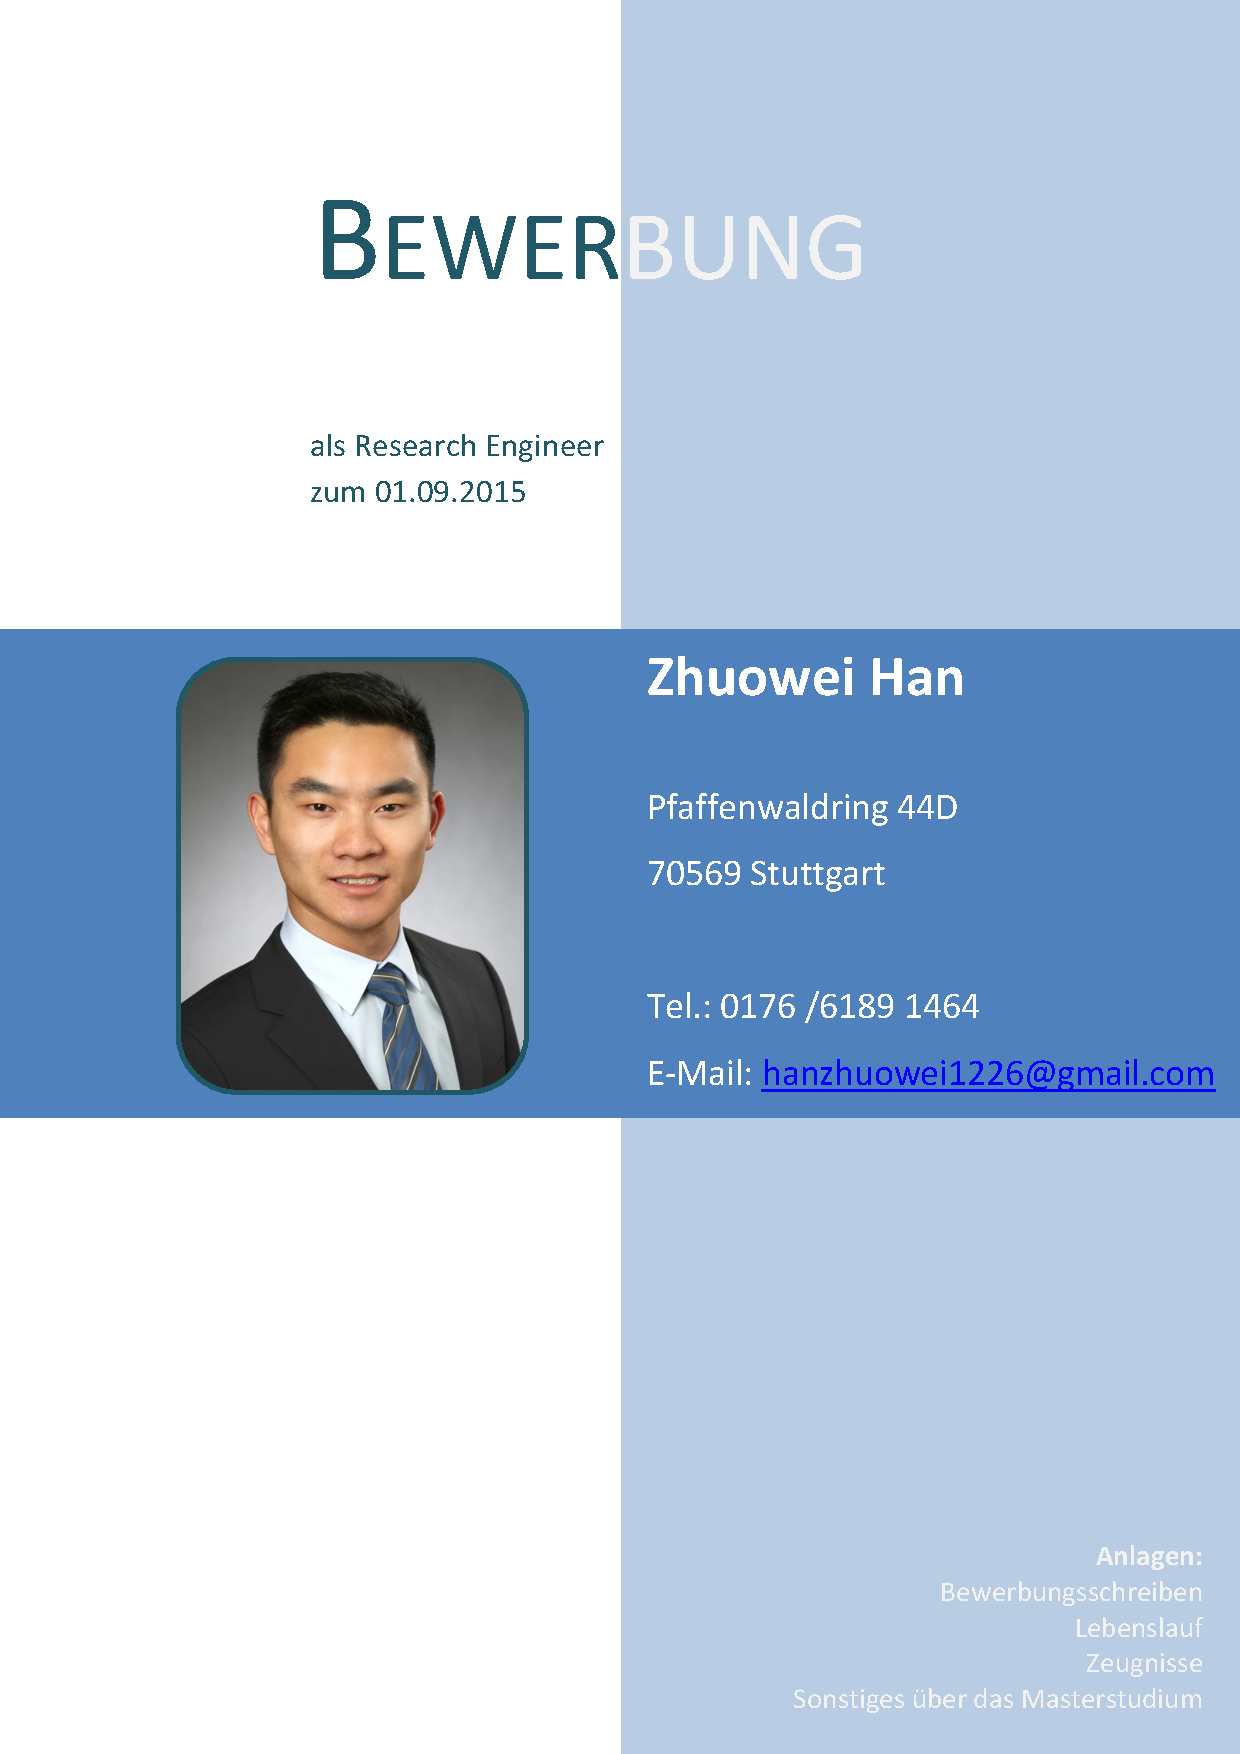
\includepdf[]{../deckblatt_STC.pdf}
%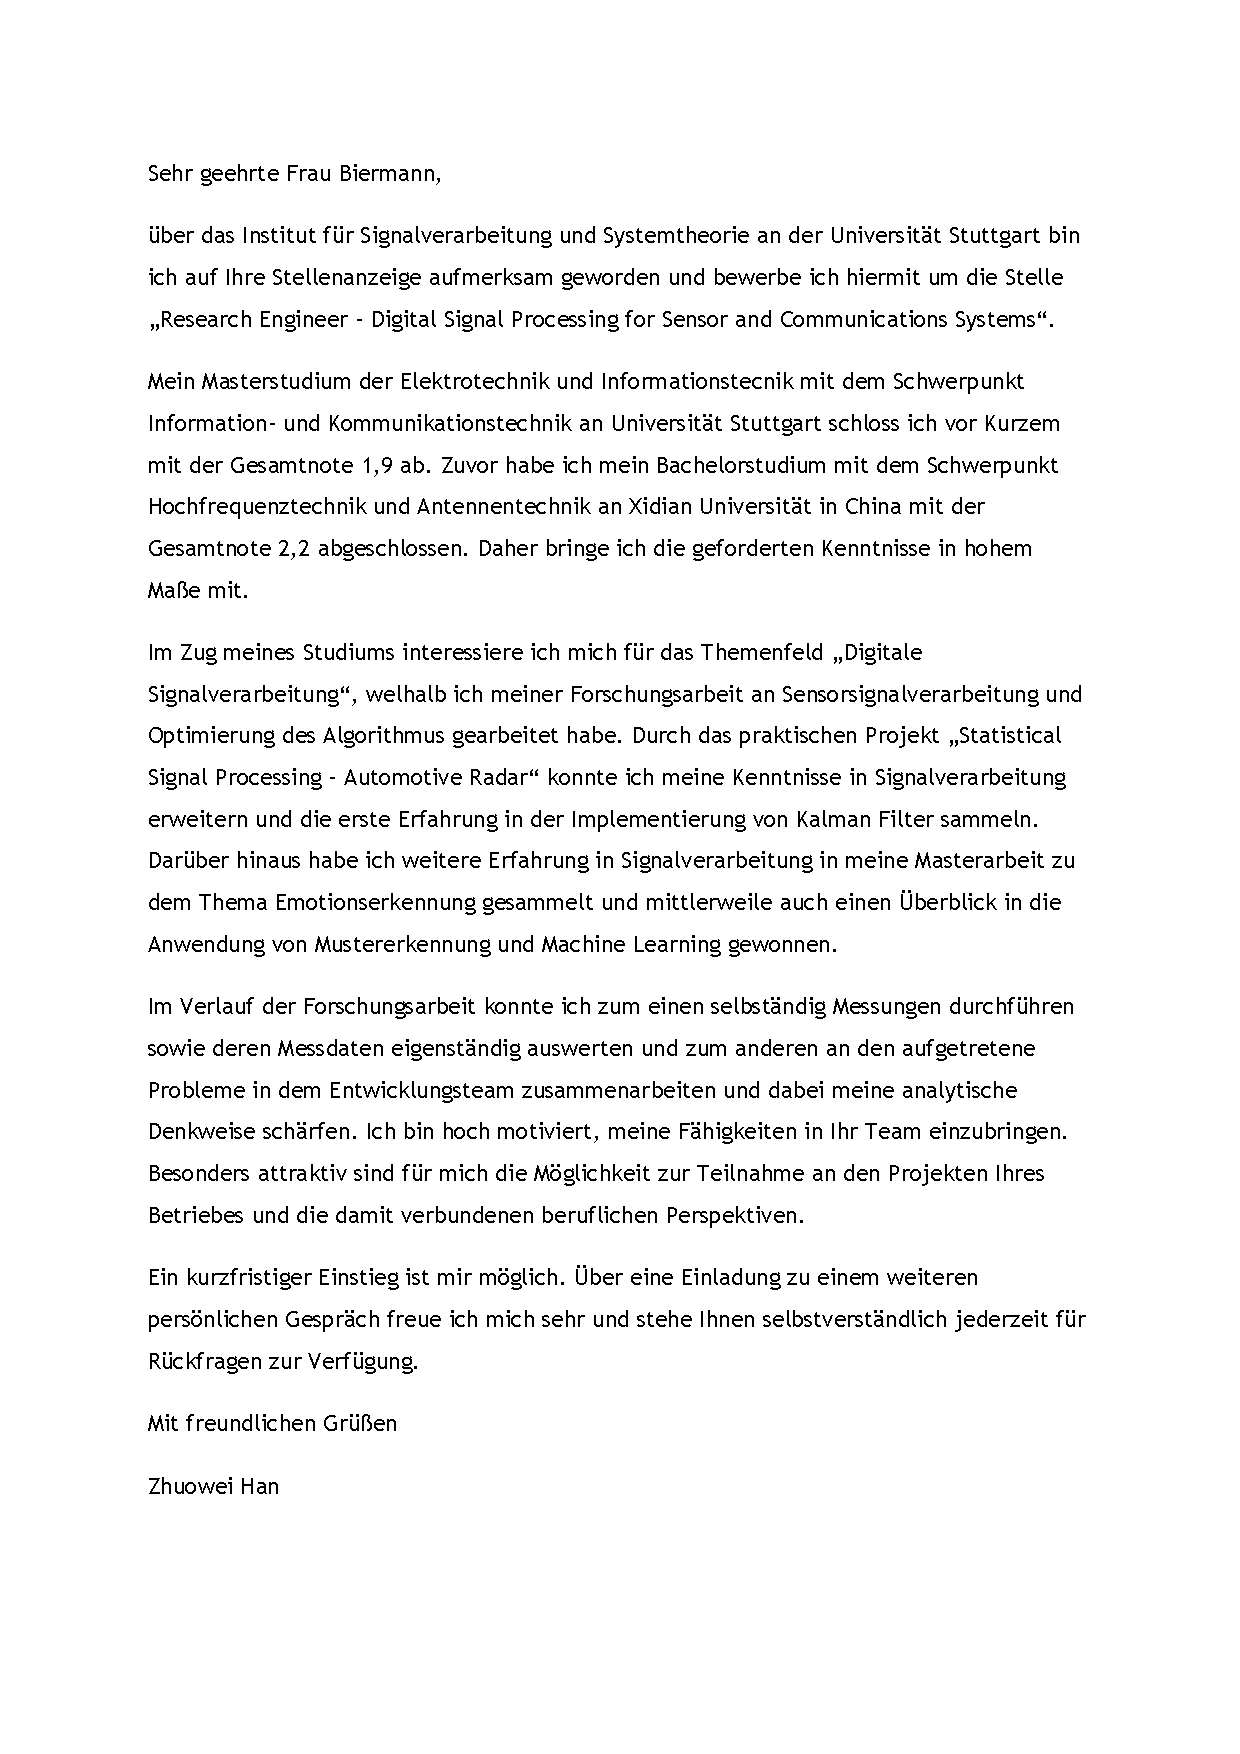
\includepdf[]{../TempAnschreiben/Signal-MachineLearning-sony.pdf}
%-----       letter       ---------------------------------------------------------
% recipient data
% \recipient{}{}
%\recipient{FERCHAU Engineering GmbH}{Niederlassung Friedrichshafen \\ Otto-Lilienthal-Straße 6\\ 88046 Friedrichshafen}
% \date{\today}
% \opening{Sehr geehrter Herr Kugler,}
% 
% %% \closing{Yours faithfully,}
% \closing{Mit freundlichen Grüßen}
% %\enclosure[Attached]{curriculum vit\ae{}}          % use an optional argument to use a string other than "Enclosure", or redefine \enclname
% \makelettertitle
% mit großem Interesse habe ich die Stellenausschreibung zum „Ingenieur Algorithmen-Entwicklung Fahrerassistenzsysteme“ gelesen und reiche Ihnen hiermit meine Bewerbungsunterlagen ein.
% 
%%Die FERCHAU Engineering GmbH als Nr.1 Deutschlands Engineering-Dienstleister stellt für mich den idealen Arbeitgeber dar. Die umfangreiche Ausrichtung des Unternehmens harmoniert ausgezeichnet mit meinem persönlichen Bestreben nach spannenden Projekten sowie innovative ausgerichtetem Denken und Agieren.
%
%Im Rahmen meiner Forschungsarbeit habe ich die erste Erfahrungen in der Algorithmenentwicklung für Fahrerassistenzsysteme und in der Sensortechnologie gesammelt. Im Verlauf der Forschungsarbeit habe ich zum einen selbständig die Messungen durchgeführt sowie deren Messdaten ausgewertet und zum anderen aufgetretene Probleme mit Arbeitskollegen diskutiert und dabei meine analytische Denkweise geschärft.
%
%Darüber hinaus konnte ich im Zuge meines Masterstudiums durch die Teilnahme am Fachpraktikum „Statistical Signal Processing – Automotive Radar“ zusätzliche Erfahrungen im Bereich Algorithmenentwicklung und Sensorsignalverarbeitung sammeln. Außerdem interessiere ich mich für das Themenfeld „Machine Learning“, weshalb ich in meiner Masterarbeit an der Emotionserkennung in Sprachsignalen gearbeitet und erfolgreich abgeschlossen habe.
%
%Ich bin hoch motiviert meine bisherigen Fachkenntnisse und Erfahrungen gezielt für die Aufgaben bei FERCHAU einzubringen. Sowohl die Möglichkeit zur Mitarbeit an den Projekten Ihres Unternehmens als auch die damit verbundenen beruflichen Perspektiven sind für mich sehr attraktiv.
% 
%Ein kurzfristiger Einstieg ist mir möglich und meine Jahresgehaltsvorstellung beträgt ca. 48,000 Euro brutto. Über eine Einladung zu einem weiteren Gespräch freue ich mich sehr und stehe Ihnen selbstverständlich jederzeit für Rückfragen zur Verfügung.
% 
% \makeletterclosing
% \clearpage
% \begin{CJK*}{UTF8}{gbsn}                          % to typeset your resume in Chinese using CJK
%%%%%%%-----       resume       ---------------------------------------------------------


\makecvtitle
\vspace{3mm}
\section{Praktische Erfahrungen}
%\subsection{Vocational}
\cventry[3pt]{09/2006 -- 04/2007}{Beijing Air Catering Co., Ltd.}{}{}{}{\begin{itemize}
\item Schwerpunkt: Technische Kundenbetreuung
\end{itemize}
}

\cventry[3pt]{10/2013 -- 02/2014}{Mazda Motor Co., Ltd}{China}{}{}{\begin{itemize}
\itemsep5pt
\item Schwerpunkt
: \begin{itemize}
\item Graphic design of racing car
\item Safety transport package of racing engine
\end{itemize}
\item Richtung: Logistik, Marketing, Außenhandel
\end{itemize}}

\cventry[3pt]{09/2012 -- 04/2013}{Shaanxi History Museum}{China}{}{}{\begin{itemize}
\itemsep5pt
\item Schwerpunkt: Safety package of precious and fragile unearthed relics
\item Richtung: Application of the 3D laser scanning and 3D printing techniques to the study of relics conservation
\end{itemize}}


\section{Ausbildung}
\cventry{09/2010 -- jetzt}{Bachelor, Verpackungstechnik}{}{\newline Hochschule der Medien}{}{}
\cventry{09/2008 -- 04/2010}{Bachelor, Staatsexamen Lebensmittelchemie}{}{\newline Universität Stuttgart}{}{}
\cventry{09/2002 -- 06/2006}{Bachelor, Bio- und Lebensmittelwissenschaft}{}{\newline Universität für Forstwirtschaft Peking}{}{}
% \section{Masterarbeit}
% \cvitem{title}{\emph{Title}}
% % \cvitem{supervisors}{Supervisors}
% \cvitem{description}{Short thesis abstract}
\section{Schulbildung}
\cventry{06/2002}{Abitur}{The Affiliated high School of Peking University}{}{}{}
\section{Sprachen}
\cvdoubleitem{Chinesisch}{Mutterspache}{}{}
\cvdoubleitem{Deutsch}{verhandlungssicher}{}{}
\cvdoubleitem{Englisch}{verhandlungssicher}{}{}
\section{Weitere Qualifikationen}
\cvitem{EDV}{MS-Office, AutoCAD, EskoCAD, Adobe Software, ANSYS}
%\cvitem{Textsatz}{\LaTeX{}}
%\cvitem{Betriebsystem}{Windows / Linux}
%\section{Hobby}
%\cvitem{}{Fotografieren, Kartfahren, Schwimmen, Klavier}

%\vspace{1cm}
%
\includegraphics[scale=0.5]{../Bild/unterschrift.png}\\
%\today, Stuttgart



%\clearpage\end{CJK*}                              % if you are typesetting your resume in Chinese using CJK; the \clearpage is required for fancyhdr to work correctly with CJK, though it kills the page numbering by making \lastpage undefined%
%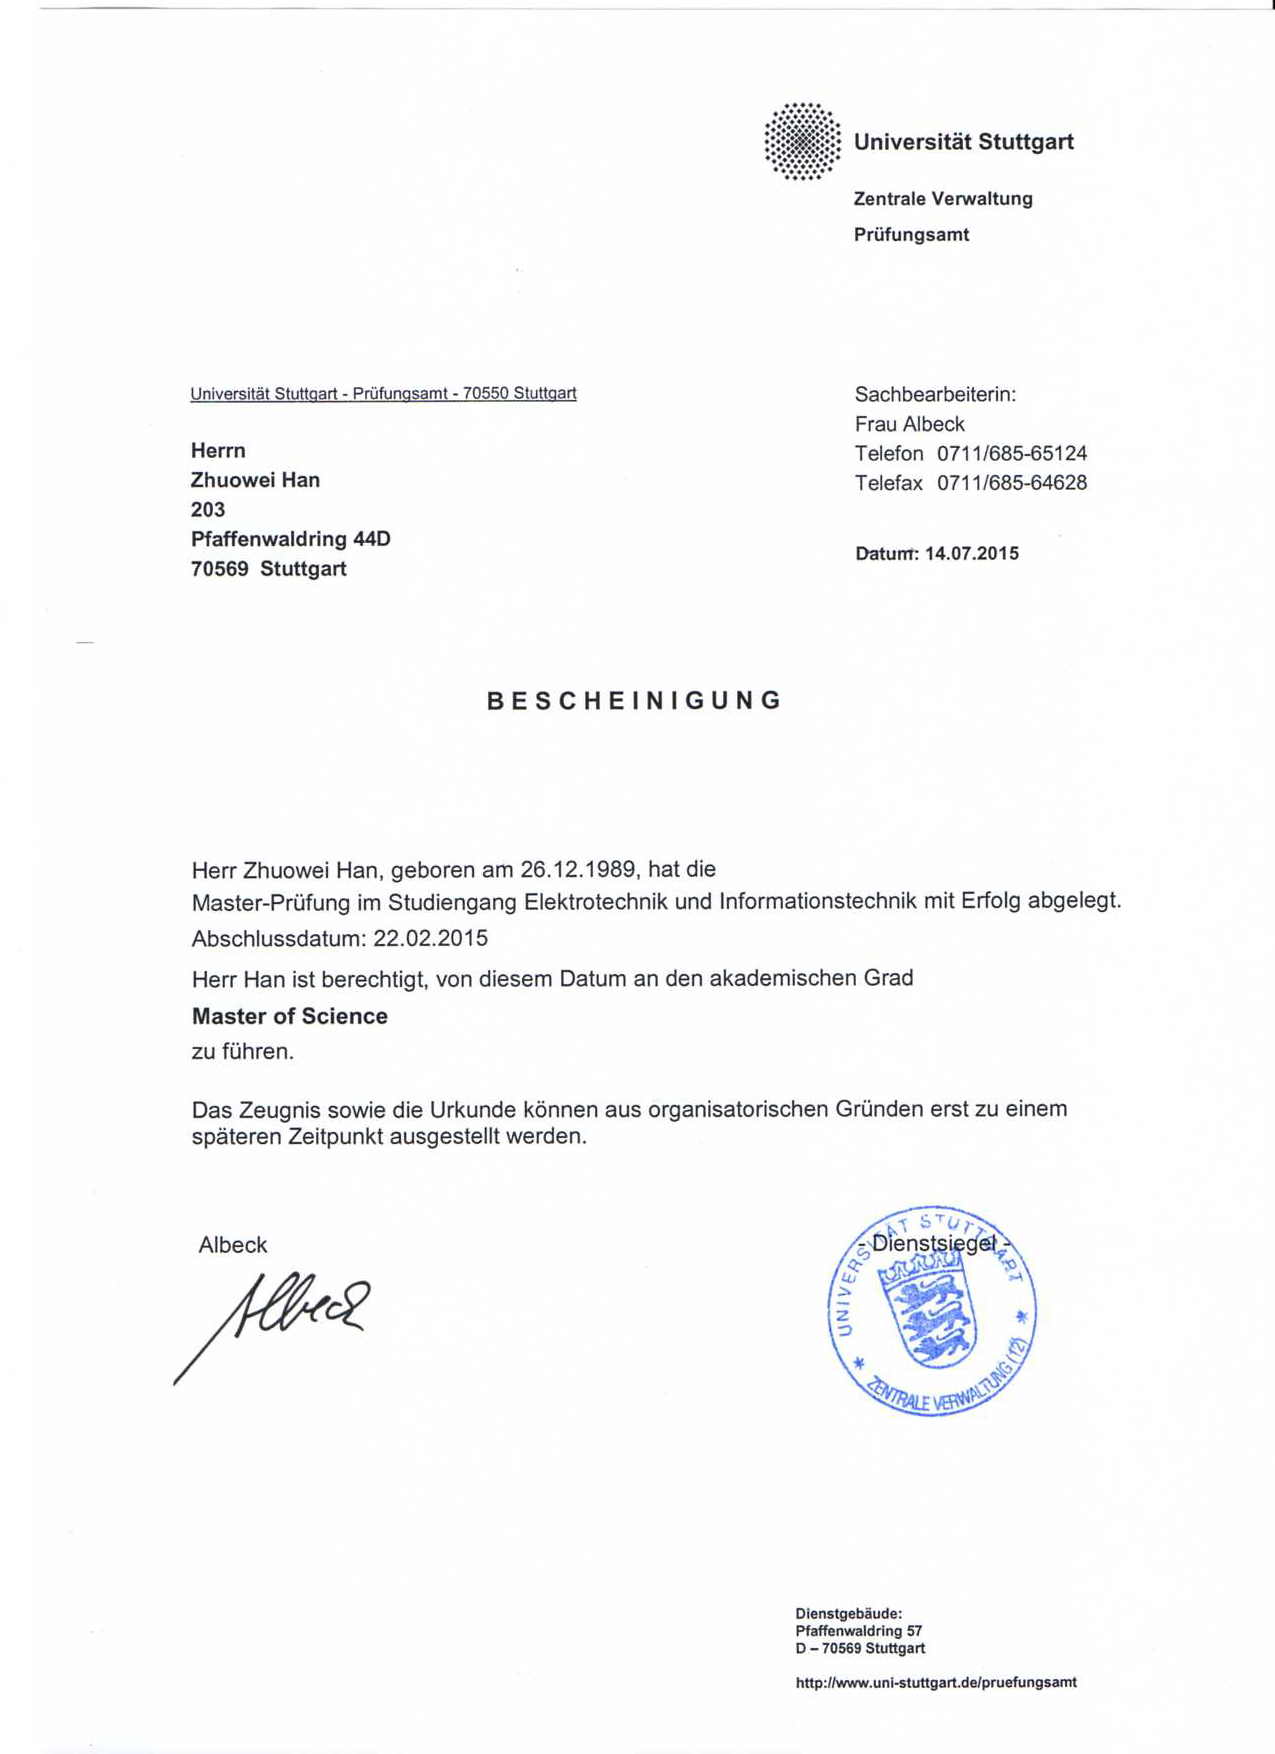
\includepdf[pages={-}]{../Certificates/Master-Bescheinigung.pdf}
%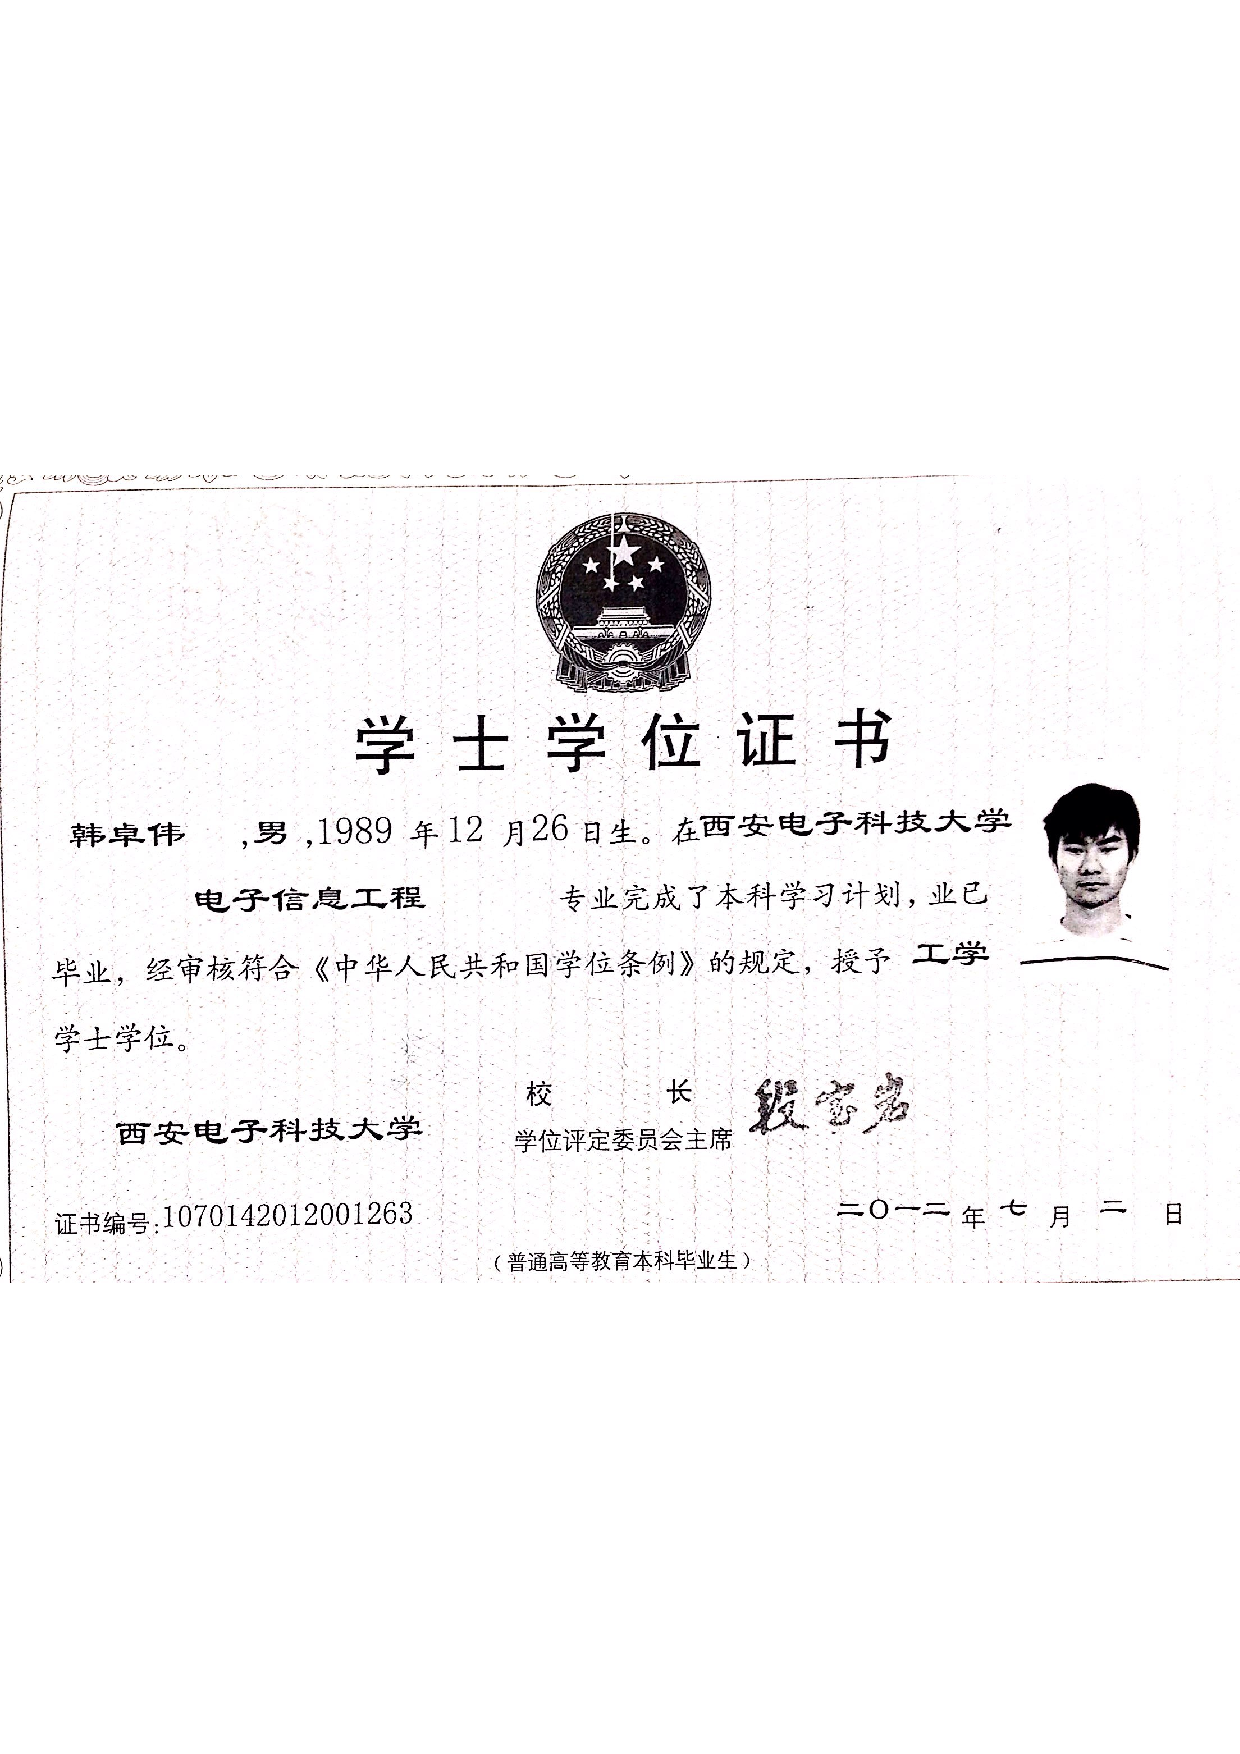
\includepdf[pages={-}]{../Certificates/BachelorUrkunde.pdf}
%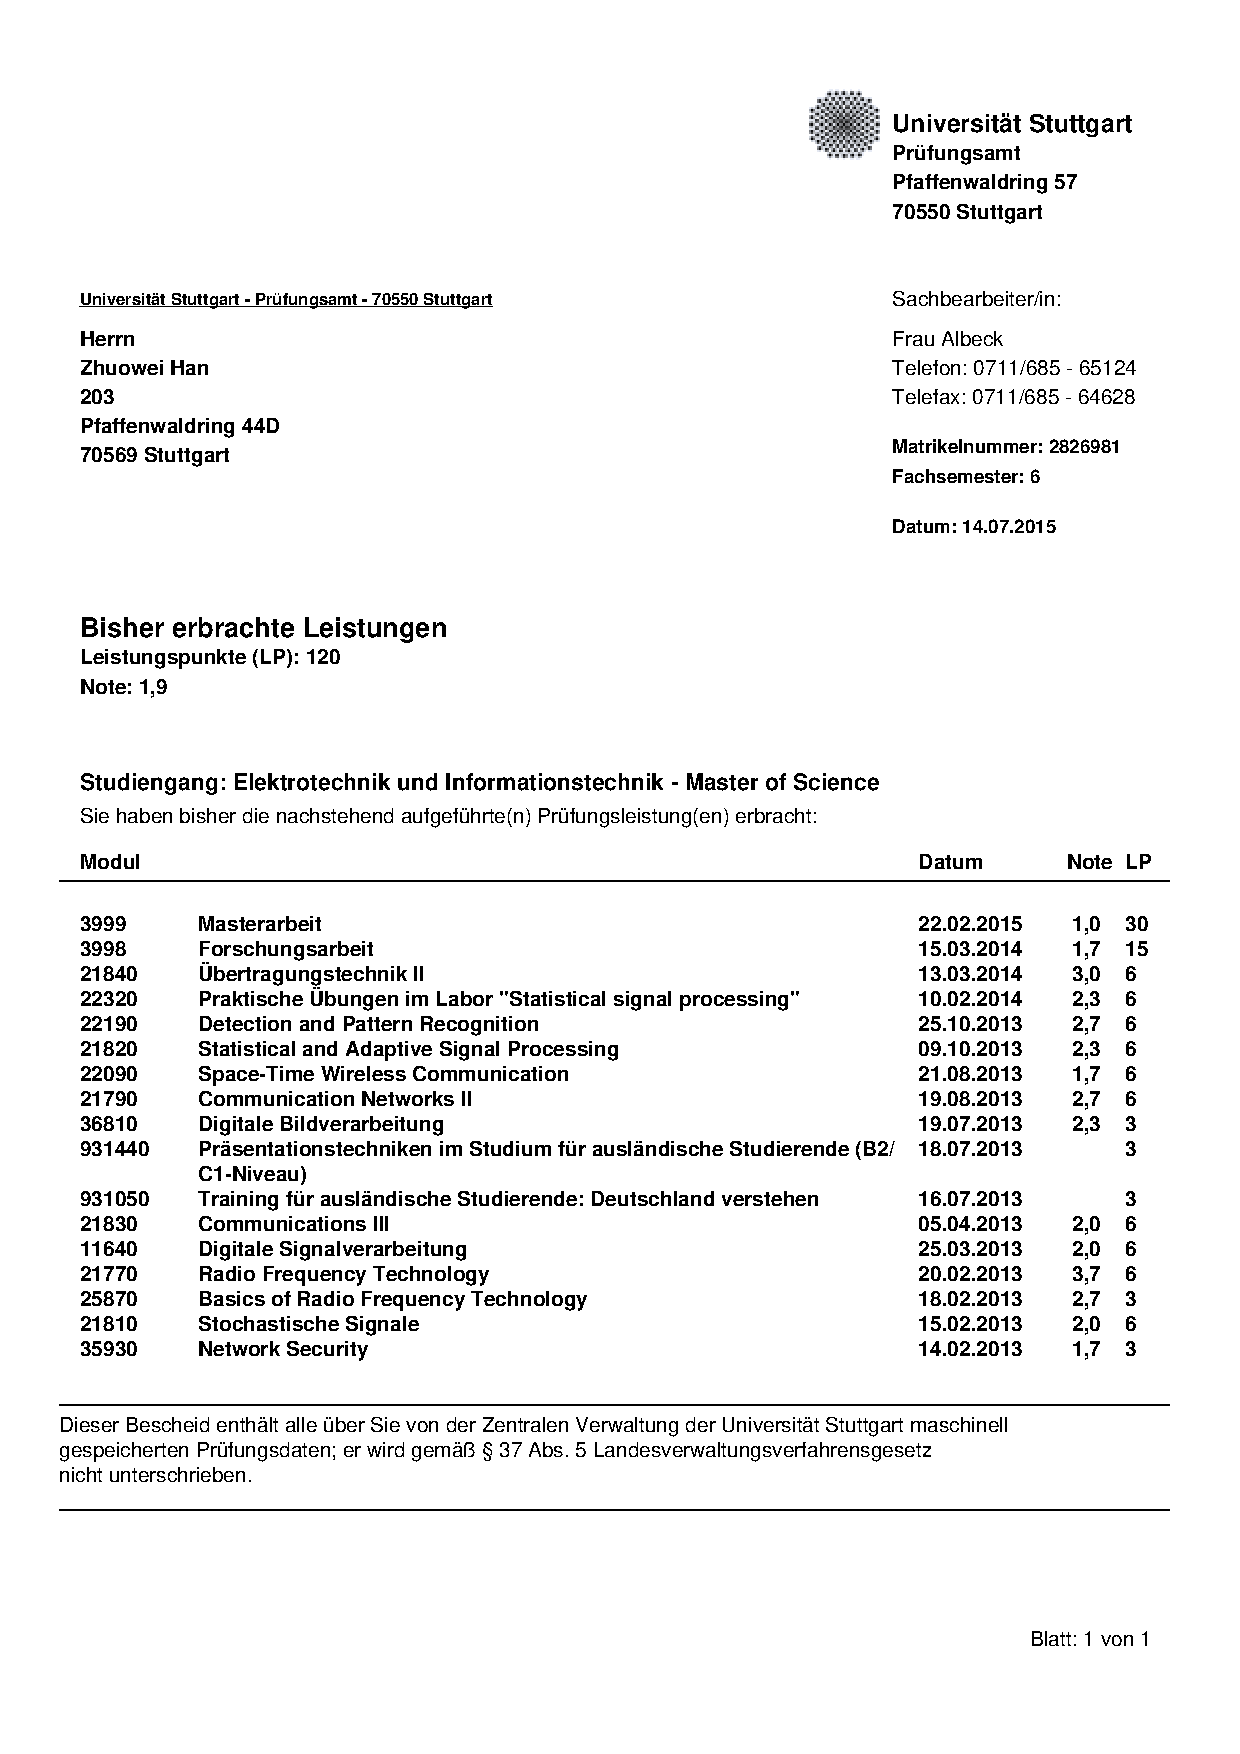
\includepdf[pages={-}]{../Certificates/Notenspiegel_Master_Han.pdf}
%
\includepdf[pages={-}]{../Certificates/presentation-masterthesis-ZhuoweiHan.pdf}
\end{document}


%% end of file `template.tex'.
